\documentclass[12pt]{niuthesis}

% line numbers for draft
\usepackage{lineno}
%\linenumbers{}

\usepackage{latexsym}
\usepackage{graphicx}
\usepackage{xspace}
\usepackage{amssymb}
\usepackage{amsmath}
\usepackage{rotating}
\usepackage{longtable}

\usepackage[
  style=numeric-comp,
  sorting=none,
  giveninits=true
]{biblatex}
\renewbibmacro{in:}{}
\bibliography{main}

\usepackage{hyperref}
\hypersetup{
  bookmarksnumbered,%
  bookmarksopen,%
  bookmarksopenlevel=1,%
  colorlinks=false,%
  pdfborder={0 0 0},%
  plainpages=false,%
  pdfencoding=auto,%
  psdextra,%
  linktoc=all,%
  pdfauthor={},%
  pdftitle={},%
  pdfsubject={},%
  pdfkeywords={your topics}%
}

\usepackage[
  nopostdot,toc,acronym,
  nomain,nonumberlist,nogroupskip
]{glossaries}

\makeatletter
\AtBeginDocument{%
  \let\thMakeUppercase\uppercase%
}
\makeatother

% Load macros and definitions
\newcommand{\twochoices}[2]{
    \left \{%
    \begin{array}{lcc}
        \displaystyle #1 \\
        \vspace{-10pt}   \\
        \displaystyle #2
    \end{array}
    \right.
}

\newcommand{\twovec}[2]{
    \left(%
    \begin{array}{c}
        #1 \\ #2
    \end{array}
    \right)
}

\newcommand{\twomatrix}[4]{
    \left(%
    \begin{array}{cc}
        #1 & #2 \\
        #3 & #4
    \end{array}
    \right)
}
\newcommand{\FASTJET}{\textsc{Fastjet}\xspace}

\newcommand{\MADGRAPH}{\textsc{MadGraph}\xspace}
\newcommand{\MCATNLO}{\textsc{mc@nlo}\xspace}
\newcommand{\MGvATNLO}{\MADGRAPH{}5\_a\MCATNLO}
\newcommand{\POWHEG}{{\textsc{powheg}}\xspace}
\newcommand{\GEANTfour}{{\textsc{Geant4}}\xspace}
\newcommand{\PYTHIA}{{\textsc{pythia}}\xspace}
\newcommand{\NanoAOD}{{\textsc{NanoAOD}}\xspace}
\newcommand{\ROOT}{{\textsc{ROOT}}\xspace}

\newcommand{\Wplusminus}{W\ensuremath{^{\pm}}}
\newcommand{\Wplus}{W\ensuremath{^{+}}}
\newcommand{\Wminus}{W\ensuremath{^{-}}}

\newcommand{\de}{\ensuremath{^\circ}}
\newcommand{\ten}[1]{\ensuremath{\times \text{10}^\text{#1}}}
\newcommand{\unit}[1]{\ensuremath{\text{\,#1}}\xspace}
\newcommand{\mum}{\ensuremath{\,\mu\text{m}}\xspace}
\newcommand{\micron}{\ensuremath{\,\mu\text{m}}\xspace}
\newcommand{\km}{\ensuremath{\,\text{km}}\xspace}
\newcommand{\m}{\ensuremath{\,\text{m}}\xspace}
\newcommand{\cm}{\ensuremath{\,\text{cm}}\xspace}
\newcommand{\mm}{\ensuremath{\,\text{mm}}\xspace}
\newcommand{\mus}{\ensuremath{\,\mu\text{s}}\xspace}

\newcommand{\seconds}{\ensuremath{\,\text{s}}\xspace}
\newcommand{\nanoseconds}{\ensuremath{\,\text{ns}}\xspace}

\newcommand{\Tesla}{\ensuremath{\,\text{T}}\xspace}

\newcommand{\sqrtOfs}{\ensuremath{\,\sqrt{s}}\xspace}

\newcommand{\keV}{\ensuremath{\,\text{ke\hspace{-.08em}V}}\xspace}
\newcommand{\MeV}{\ensuremath{\,\text{Me\hspace{-.08em}V}}\xspace}
\newcommand{\GeV}{\ensuremath{\,\text{Ge\hspace{-.08em}V}}\xspace}
\newcommand{\TeV}{\ensuremath{\,\text{Te\hspace{-.08em}V}}\xspace}

\newcommand{\fbinv}{\mbox{\ensuremath{\,\text{fb}^{-1}}}\xspace}
\newcommand{\pbinv}{\mbox{\ensuremath{\,\text{pb}^{-1}}}\xspace}

\newcommand{\lumi}{\ensuremath{\mathcal{L}}\xspace}

\newcommand{\LLow}{\ensuremath{\mathcal{L}=\text{10}^\text{33}\,\text{cm}^\text{\(-\)2}\,\text{s}^\text{\(-\)1}}\xspace}
\newcommand{\LMed}{\ensuremath{\mathcal{L}=\text{2}\times \text{10}^\text{33}\,\text{cm}^\text{\(-\)2}\,\text{s}^\text{\(-\)1}}\xspace}
\newcommand{\LHigh}{\ensuremath{\mathcal{L}=\text{10}^\text{34}\,\text{cm}^\text{\(-\)2}\,\text{s}^\text{\(-\)1}}\xspace}

\newcommand{\pt}{\ensuremath{p_{\mathrm{T}}}\xspace}
\newcommand{\ET}{\ensuremath{E_{\mathrm{T}}}\xspace}
\newcommand{\HT}{\ensuremath{H_{\mathrm{T}}}\xspace}
\newcommand{\mT}{\ensuremath{m_{\mathrm{T}}}\xspace}

\newcommand{\CL}{\ensuremath{\text{CL}}\xspace}
\newcommand{\CLs}{\ensuremath{\text{CL}_\text{s}}\xspace}
\newcommand{\CLsb}{\ensuremath{\text{CL}_\text{s+b}}\xspace}


% Load glossary and set style
\makeglossaries{}
\newglossarystyle{mylong}{
  \setglossarystyle{long}
  \renewenvironment{theglossary}%
  {\setlength\LTleft{0pt}
   \setlength\LTright{0pt}
   \setlength{\glsdescwidth}{0.85\linewidth}
   \begin{longtable}{@{}lp{\glsdescwidth}@{}}}%
  {\end{longtable}}
  \renewcommand*{\glsgroupskip}{}
}
\setglossarystyle{mylong}
\setacronymstyle{long-short}
\loadglsentries{glossary}

% List of Symbols
\newcommand{\listofXXX}{% List of Acronyms
\glsaddall{}
\printglossary[
  title=List of Acronyms,
  type=\acronymtype,
]

% \chapter*{List of Blah}
% \addcontentsline{toc}{chapter}{List of Blah}}

\begin{document}

\title{Search for Vector Boson Scattering in semileptonic decay channel using CMS Experiment}

\author{Ramanpreet Singh}

\major{Physics}
\degree{Dissertation}{Ph.D.}{Doctor of Philosophy}
\degreedate{September}{2021}
\department{Department of Physics}
\director{Vishnu Zutshi}

\begin{abstract}
  This dissertation reports on the search for
the \gls{VBS} in semileptonic channel \textit{ZV},
where the \textit{Z} boson decays to a pair of leptons (electrons or muons),
and the other vector boson \textit{V} (either \textit{W} or \textit{Z})
decays hadronically to a pair of jets, in association of two jets
i.e.~\( \textit{ZV}jj \rightarrow l^{+}l^-jjjj \), \( l=e \) or \( \mu \).
The search used 137 \fbinv{} of proton-proton collision data collected by
the \gls{CMS} experiment at the \gls{LHC} with
center-of-mass energy (\( \sqrt{s} \)) of 13 \TeV{} from 2016 to 2018.
\gls{VBS} is a key process in understanding the nature of \gls{EWSB} in
the framework of \gls{SM}.

Studies and instrumentation done towards the future detector
upgrade to the \gls{CMS} experiment which will replace
the current endcap \gls{HCAL} and \gls{ECAL} with \gls{HGCAL}
during \gls{LS3} are also reported.
Optimal configuration
of scintillator tiles coupled to \glspl{SiPM}
in the \gls{HGCAL} is measured and suggested using testbeam measurement of
scintillator tiles and noise measurement of \glspl{SiPM}.
Prototyping of automated wrapping of scintillator tiles in \gls{ESR} film
are also discussed.

\end{abstract}

\begin{acknowledgments}
  First, I would like to thank my advisor, Vishnu Zutshi
for giving me opportunities to make this work possible.
Your mentorship and guidance over the last six years has
contributed to my growth as a scientist and as a person. Thank you
for all the discussions and being patient with me.
I would also like to thank my committee members Michael (Mike) Eads,
Gerald (Jerry) Blazey, and Jeffrey Berryhill for providing feedback
on my dissertation.

For the analysis, I would like to thank Michael (Mike) Eads, for providing
guidance and suggestions throughout the analysis.
I would also like thank Jeffrey Berryhill, Aram Apyan, Jay Lawhorn
and CMS collaboration for their help and guidance.


I would like to thank Alexandre (Sasha) Dychkant for
teaching me various lab equipments and sharing his experimental knowledge.
I would also like to thank
Iman Salehinia, Nicholas Pohlman, Michael Figora, Todd Fletcher,
and Brian Scott who made the instrumentation of
scintillator tile wrapping machine possible.

I would like to thank NIU physics faculty and staff. I would also
like to thank my fellow graduate students
Prudhvi Raj Varma Chintalapati,
Christina Sarosiek,
Brendan Leung,
Aakaash Narayanan,
Osama Mohsen,
Ben Simons,
Wei Hou Tan,
Austin Dick,
Andrew Best,
Prudhvi Nikhil Bhattiprolu,
Will Baker,
Kevin Hamilton,
Jeremiah Mitchell,
and Sebastian Szustkowski
for being great friends.


Lastly, I would like to thank my family for their constant
support and love throughout my time away from home.
\end{acknowledgments}

\begin{dedication}
  I dedicate this dissertation to my mother, \textit{Harsharan Kaur};
my father, \textit{Lakhmir Singh};
and my brother; \textit{Gurpreet Singh} for their love and support.
\end{dedication}

% Make Prologue
\MakeThesisPrologue{}

% Reset glossary acronyms
\glsresetall{}

% Chapters
\chapter{
  Introduction
 }\label{ch_intro}

\epigraph{\textit{It doesn't matter how beautiful your theory is,
    it doesn't matter how smart you are. \\
    If it doesn't agree with experiment, it's wrong.
    In that simple statement is the key to science.}}
{--- Richard P. Feynman}

``Particle Physics'' is the branch of physics which deals with the fundamental
particles and the interactions between them. Fundamental particles are the
subatomic particles which are not made of other particles.
There are two types of fundamental particles ``matter'' and ``interaction''
particles, as the name suggests matter particles are the fundamental constituent of matter and
the interactions between among them is governed by how they exchange interaction particles.
\gls{SM} of particle physics is the theory that classifies these fundamental
particles and describes three out of four fundamental
interaction forces; electromagnetic, weak, and strong.

This chapter introduces briefly to the theory of \gls{SM}, Higgs mechanism,
spontaneous \gls{EWSB}, \gls{VBS}, and the motivation for the search of \gls{VBS}
in semileptonic decay channel ZV with leptonic decay of Z,
and hadronic decay of V (W/Z) to pair of quarks.

\section{
  Standard model
 }\label{ch_intro:standard-model}

In \gls{SM}, the matter particles are fermions, and
the interaction particles are bosons. \gls{SM} also includes
anti-fermions, which are fermions with equal mass but opposite sign of charge.
Figure~\ref{fig:standard-model-details} lists mass, electric charge,
and spin of fermions and bosons in \gls{SM}.

Fermions obey Fermi-Dirac statistics and have half integer spin. They can be further
divided into leptons which have integral electric charge, and quarks which have
fractional electric charge. There are three generations of quarks and leptons
discovered to the date, each generation only differs by the mass.
In addition to the electric charge, quarks also have
three types of ``color'' charge (red, green and blue). Quarks cannot be isolated
because of ``color confinement'', which requires net color charge to be zero
for an isolated particle, for this reason we can only have certain composition
of quarks. Baryons (proton, neutrons, etc.) are made up of three quarks with
each with different color charge,
and mesons (pions, kaons, etc.) are made of two quarks with color and anti-color charge.

Bosons obey Bose-Einstein statistics and have integral spin.
They are described by local gauge theory and are also called gauge boson.
Photons are the interaction particle of electromagnetic force, they are massless
and only interact with charged particles. Gluons are the mediator of strong force
between quarks, they are massless and carries color charge. \Wplusminus{} and Z
are the vector bosons and mediator of weak force,
unlike photons and gluons they are massive. \Wplus{} and \Wminus{}
are antiparticles of each other, and Z is antiparticle of its own.
The last gauge boson Higgs is a massive scalar boson with zero spin,
zero electric and color charge. Higgs boson is not a force carrier,
but rather explains why only some particles have mass.

The \gls{SM} is built in the framework of \gls{QFT}, in which particles
are excitation of the fields and interactions arise from local gauge
invariance. The \gls{SM} is a \( {SU(3)}_C \otimes {SU(2)}_L \otimes {U(1)}_Y\)
gauge theory, \( {U(1)}_Y \), \( {SU(2)}_L \), \( {SU(3)}_C \) are the gauge symmetries
of \gls{QED}, weak interaction and \gls{QCD} respectively, where the indices
stands for ``hypercharge'' (Y), ``left-handed'' (L) and ``color'' (C).

\begin{figure}[!ht]
  \centering
  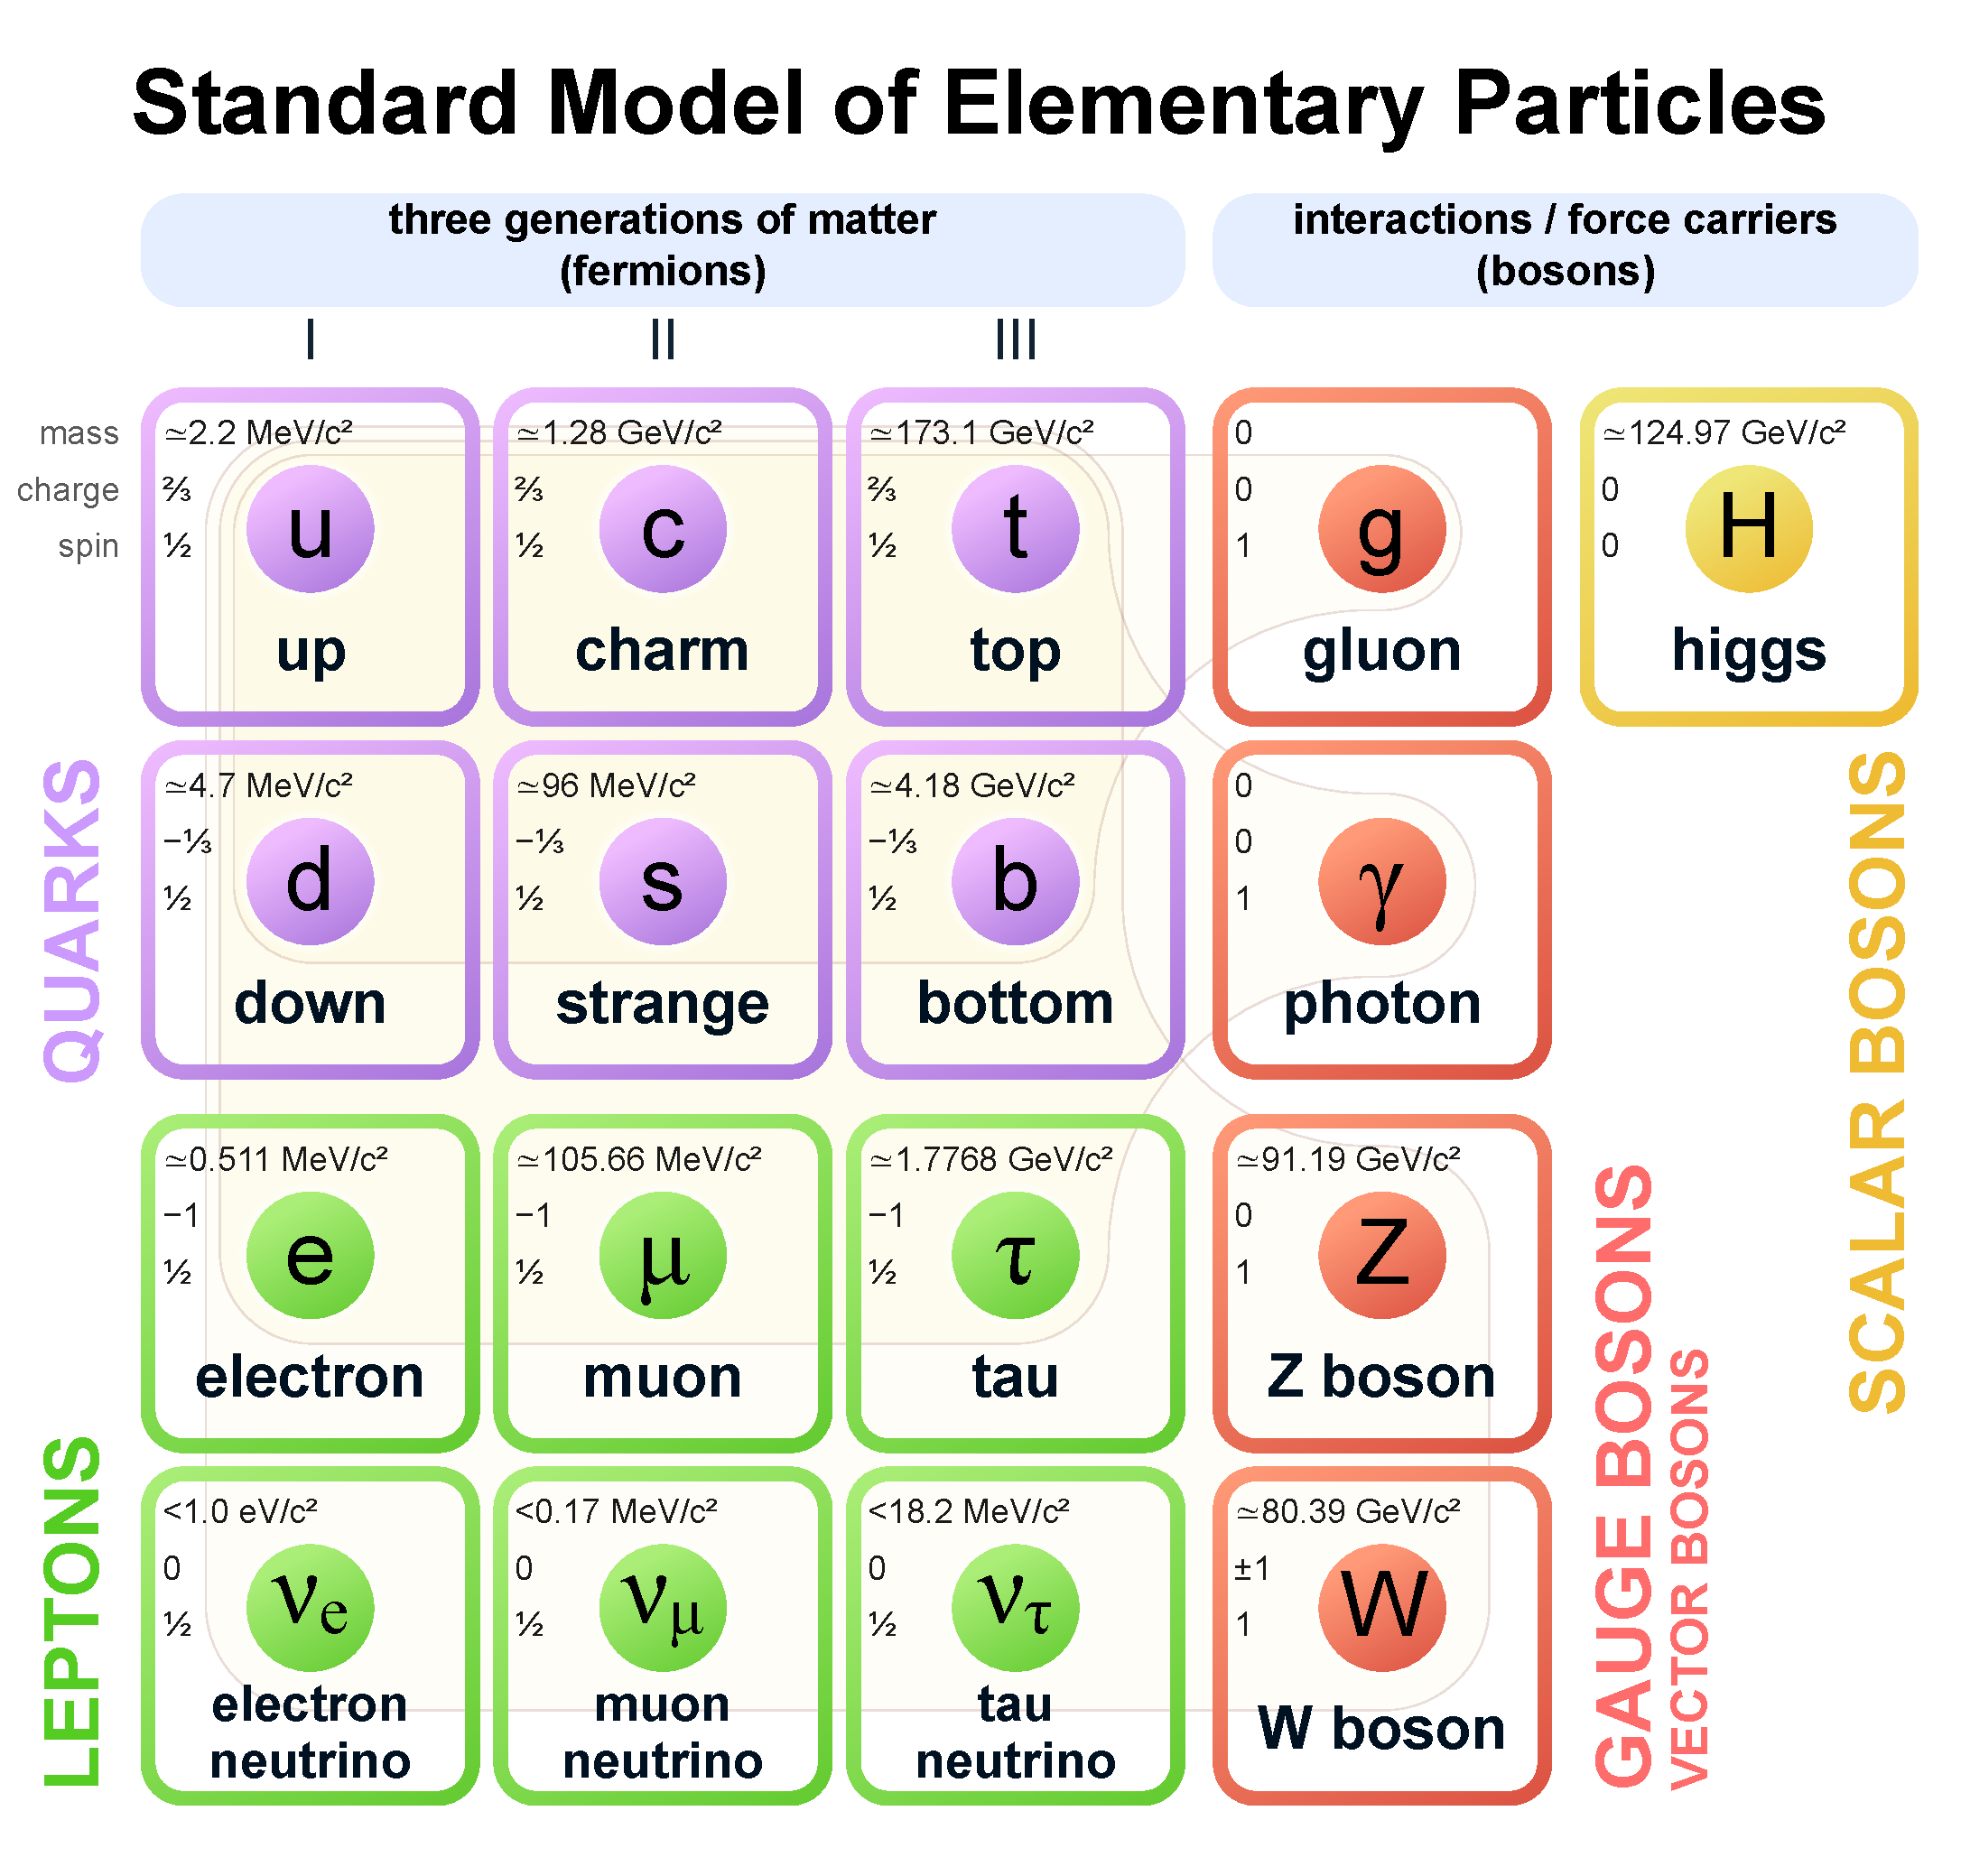
\includegraphics[width=0.8\textwidth]{figures/Standard_Model_of_Elementary_Particles.pdf}
  \caption[Standard model list of matter and interaction particles]%
  {Standard model list of matter and interaction particles~\cite{image-standard-model}}%
  \label{fig:standard-model-details}
\end{figure}

\subsection{
  Quantum Electrodynamics (QED)
}\label{ch_intro:qed}

\gls{QED} is a quantum field theory of electrodynamics, it describes
the interaction of photons to the charged fermions.
The \gls{QED} is local gauge invariant and symmetric with \( {U(1)}_{Q} \) group,
defined as,
%
\begin{align}
  {U(1)}_{Q} = \exp\left( { i Q \theta (x) } \right)
\end{align}

where \( \theta (x) \) is any spacetime function also called gauge parameter,
and \( Q \) is coupling constant of photon field to the fermions
which is equivalent to the charge of fermion.

Under this transformation, fermion spinor \( \psi (x) \) and
four-potential \( A_{\mu} \) electromagnetic tensor will transform
as,
%
\begin{align}
  \psi (x) \rightarrow {U(1)}_{Q} \psi (x) \\
  A_{\mu} \rightarrow A_{\mu} - \frac{1}{e} \partial_{\mu} \theta
\end{align}

The general Lagrangian of \gls{QED} for fermions and their interaction
with photon field is given by,
%
\begin{equation}\label{eq:lag-qed}
  {\mathcal{L}}_{QED} = \bar{\psi} ( i {\gamma}^{\mu} {D}_{\mu} - m ) \psi
  - \frac{1}{4} {F}_{\mu \nu} {F}^{\mu \nu}
\end{equation}

where \( m \) is the mass of fermion,
\( {D}_{\mu} \) is the covariant derivative,
and \( {F}_{\mu \nu} \) is the electromagnetic field tensor defined as,
%
\begin{align}
  {D}_{\mu} = \partial_{\mu} + i Q A_{\mu} \\
  {F}_{\mu \nu} = \partial_{\mu} A_{\nu} - \partial_{\nu} A_{\mu}
\end{align}

\subsection{
  Quantum Chromodynamics (QCD)
}\label{ch_intro:qcd}

The strong interactions are represented by \( {SU(3)}_{C} \) gauge group, invariant
under transformations of color charge degree of freedom, and it is based
on Yang-Mills theory~\cite{Yang-Mill:1954}. Since ``electrodynamics''
is the theory of electric charge, this theory of color (\textit{chromo} in Greek)
charge is called ``chromodynamics'', hence the name \glsfirst{QCD}.

A quark spinor in initial state can be represented as,
%
\begin{equation}
  \psi = \left( \begin{matrix}
    \psi_{red}  \\
    \psi_{blue} \\
    \psi_{green}
  \end{matrix} \right)
  = \left( \begin{matrix}
    \psi_{1} \\
    \psi_{2} \\
    \psi_{3}
  \end{matrix} \right)
\end{equation}

\( {SU(3)}_{C} \) is an exact symmetry, it means the difference between
colors cannot be measured experimentally, thus the color labels in quark spinor are arbitrary.
\( {SU(3)}_{C} \) transformation is defined as,
%
\begin{equation}
  {SU(3)}_{C} = \exp \left( {i \theta^{a}(x) \frac{\lambda^{a}}{2}} \right)
\end{equation}

where \( \lambda^{a} \) for \( a = 1,\ldots,8\),
are the Gell-Mann matrices, and \( \theta^{a}(x) \) are any gauge parameters.
These eight generators of symmetry corresponds to eight gauge vector boson gluons.

Similar to \gls{QED}, the covariant derivative for \gls{QCD} can be formed as,
%
\begin{equation}
  D_{\mu} = \partial_{\mu} + i g_s \frac{\lambda^{a}}{2} G_{\mu}^{a}
\end{equation}

where \( g_s \) is the coupling constant of gluon to the quarks,
and \( G_{\mu}^{a} \) are the eight gauge fields corresponding to gluons.

Now the corresponding field strength tensor in \gls{QCD} can be formed as,
%
\begin{equation}
  F_{\mu \nu}^{a} = \partial_{\mu} G_{\nu}^{a} - \partial_{\nu} G_{\mu}^{a}
  - g_s f^{abc} G_{\mu}^{b} G_{\nu}^{c}
\end{equation}

where \( f^{abc} \) are the structure constants of \( {SU(3)}_{C} \)
which satisfy \( [\lambda^{a}, \lambda^{b}] = i f^{abc} \lambda^{c} \) relation.

The full Lagrangian for \gls{QCD} can now be constructed as,
%
\begin{equation}
  {\mathcal{L}}_{QCD} = {\bar{\psi}}^{i}
  ( i {\gamma}^{\mu} {{D}_{\mu}}^{ij} - m \delta^{ij} )\psi^{j}
  - \frac{1}{4} {F}_{\mu \nu}^{a} {F}^{a \mu \nu}
\end{equation}

for mass \( m \), indices \( i \) and \( j \) runs from 1 to 3.

The main difference of gluon field with respect to photon field is
the presence of third term in
field strength tensor which allows triplet and quartic
self coupling of gluons.

\subsection{
  Electroweak Theory
}\label{ch_intro:ew}

The theory of weak interaction which changes the flavor of fermions is
called \gls{QFD}. Since the unification of electromagnetic
and weak interaction into \gls{EW} interaction by
Glashow, Weinberg, and Salam~\cite{Glashow1959,Weinberg1967,Salam1959},
the weak interaction is better understood in terms of \gls{EW} theory.

Weak interaction only couples to left-handed fermions and it is same
whether the fermion is charged or not. The underlying gauge group of
\gls{EW} interaction is \( {SU(2)}_{L} \otimes {U(1)}_{Y} \) and
has two transformations one for the left-handed doublet
\( L \) and the right handed singlet fermions \( \psi_R \) which are defined as,
%
\begin{align}
  {SU(2)}_{L} \otimes {U(1)}_{Y} & =
  \exp \left( {i \theta^{a}(x) \frac{\sigma^a}{2}} + {i \theta(x) \frac{Y}{2}} \right)
  , \quad (doublet)                                                                \\
                                 & = \exp \left( {i \theta(x) \frac{Y}{2}} \right)
  , \quad (singlet)
\end{align}

where \( Y \) is the hypercharge (linear combination of electric charge and weak
isospin component), and \( \sigma^{a} \) for \( a = 1,2,3 \)
are the Pauli spin matrices generator of \( SU(2) \) symmetry. Left-handed
fermion \( L \) doublets are,
%
\begin{equation}
  L = \left(\begin{matrix}
    \nu_e \\
    e_L
  \end{matrix}\right) ,
  \left(\begin{matrix}
    \nu_\mu \\
    \mu_L
  \end{matrix}\right) ,
  \left(\begin{matrix}
    \nu_\tau \\
    \tau_L
  \end{matrix}\right) ,
  \left(\begin{matrix}
    u_L \\
    d_L
  \end{matrix}\right) ,
  \left(\begin{matrix}
    c_L \\
    s_L
  \end{matrix}\right) ,
  \left(\begin{matrix}
    t_L \\
    b_L
  \end{matrix}\right)
\end{equation}

and right-handed singlets are,
%
\begin{equation}
  \psi_R = e_R, \mu_R, \tau_R, u_R, d_R, c_R, s_R, t_R, b_R
\end{equation}

The covariant
derivative of \gls{EW} is then,
%
\begin{align} \label{eq:ew-dmu}
  D_{\mu} L      & = \left( \partial_{\mu} + i g_w \frac{\sigma^{a}}{2} W^{a}_{\mu} + i g \frac{Y}{2} B_{\mu} \right) L \\
  D_{\mu} \psi_R & = \left( \partial_{\mu} + i g \frac{Y}{2} B_{\mu} \right) \psi_R
\end{align}

where \( W^{a}_{\mu} \) and \( B_{\mu} \) are the gauge fields. The \gls{EW}
Lagrangian can now written as,
%
\begin{align}
  \mathcal{L}_{EW} = i \bar{L} \gamma^{\mu} D_{\mu} L
  + i \bar{\psi}_R \gamma^{\mu} D_{\mu} \psi_R
  - \frac{1}{4} {W}_{\mu \nu}^{a} {W}^{a \mu \nu}
  - \frac{1}{4} {B}_{\mu \nu} {B}^{\mu \nu}
\end{align}

where \( B_{\mu \nu} \) and \( W^{a}_{\mu \nu} \) are fields strength,
defined as,
%
\begin{align}
  B_{\mu \nu }    & = \partial_{\mu} B_{\nu} - \partial_{\nu} B_{\mu}         \\
  W_{\mu \nu}^{a} & = \partial_{\mu} W_{\nu}^{a} - \partial_{\nu} W_{\mu}^{a}
  - g_w \epsilon^{abc} W_{\mu}^{b} W_{\nu}^{c}
\end{align}

the linear combination of \( B_{\mu} \) and \( W_{\mu} \) gauge field, with a weak mixing
angle \( \theta_w \) gives 4 vectors boson \Wplus, \Wminus, Z, and \( \gamma \) of \gls{SM},
%
\begin{align}
  W^{\pm}_{\mu} & = \frac{1}{\sqrt{2}} \left( W^{1}_{\mu} \mp W^{2}_{\mu} \right) \\
  Z_{\mu}       & = \cos \theta_w W^{3}_{\mu} - \sin \theta_w B_{\mu}             \\
  A_{\mu}       & = \sin \theta_w W^{3}_{\mu} + \cos \theta_w B_{\mu}             \\
  \tan \theta_w & = g/g_{w}
\end{align}

Similar to \gls{QCD}, the presence of third term in field strength tensor
allows the self triple (WWZ, WW\( \gamma \)) and quartic (WWWW, WWZZ,
WWZ\( \gamma \), WW\( \gamma \gamma \)) couplings.

\subsection{
  Electroweak Symmetry Breaking and Higgs Mechanism
}\label{ch_intro:ewsb}

The \textit{spontaneous symmetry breaking} is the phenomena which explains
why the ground state is not invariant under the symmetry
of the Lagrangian. The ``spontaneous'' means the symmetry
breaking is not done by external agent but rather by Lagrangian itself
in ground state.

The \gls{EW} theory unifies weak interaction and \gls{QED} but the
gauge boson in \gls{EW} theory are all massless, if we were to add mass
terms like \( - m^{2} W_{\mu} W^{\mu} \) by hand, it will no longer
be gauge invariant. The solution to this without breaking gauge invariance
is spontaneous symmetry breaking, but this requires addition of new scalar
field called Higgs field via \gls{BEH}~\cite{Englert1964,Higgs1964}, and this
symmetry breaking is known as \glsfirst{EWSB}.

\gls{BEH} introduces a complex scalar field as \( {SU(2)}_L \)
doublet with non-zero \gls{VEV},
%
\begin{equation}
  \phi = \left( \begin{matrix}
      \phi^{+} \\
      \phi^{0}
    \end{matrix} \right)
  = \frac{1}{\sqrt{2}}
  \left( \begin{matrix}
      \phi^{1} + i \phi^{2} \\
      \phi^{3} + i \phi^{3}
    \end{matrix} \right)
\end{equation}

and \gls{BEH} Lagrangian is,
%
\begin{equation}
  \mathcal{L}_{BEH} = {| D_{\mu} \phi |}^{2} - V(\phi)
\end{equation}

where \( D_{\mu} \) is same as \gls{EW} covariant derivate
in Equation~\ref{eq:ew-dmu}, and \( V(\phi) \) is,
%
\begin{equation}
  V(\phi) = \mu^{2} |\phi|^{2} + {\lambda (|\phi|^{2})}^{2}
\end{equation}

the parameter \( \lambda \) is required to be positive,
for \( \mu^2 > 0\) the minima is at 0, which is not an interesting case,
but for \( \mu^2 < 0\) vacuum state energy is given by,
%
\begin{equation}
  \phi^{\dagger} \phi = - \frac{\mu^{2}}{2 \lambda}
\end{equation}

by the choice of non-zero \gls{VEV} \( v \), scalar field can be parameterized as,
%
\begin{align}
  v        & = \sqrt{\frac{- \mu^2}{\lambda}}                 \\
  \phi (x) & = \frac{1}{\sqrt{2}} \left( \begin{matrix}
                                             0 \\
                                             h (x) + v
                                           \end{matrix} \right)
\end{align}

where \( h(x) \) is the Higgs field and \gls{BEH} spontaneously breaks electroweak symmetry,
%
\begin{equation}
  {SU(2)}_L \otimes {U(1)}_Y \rightarrow {U(1)}_{EM}
\end{equation}

Visually the Higgs potential is shown in Figure~\ref{fig:higgs-potential}. The ball position
at the center represents unbroken symmetry, and at the minima represents spontaneous
broken symmetry in the ground state of potential.
%
\begin{figure}[!ht]
  \centering
  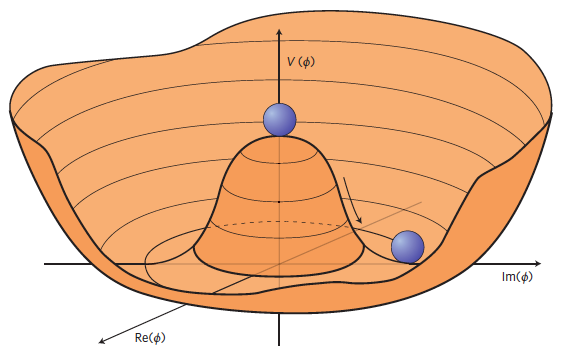
\includegraphics[width=0.7\textwidth]{figures/higgspotential.png}
  \caption[3D representation of Higgs potential]%
  {3D representation Higgs potential~\cite{image-higgs-potential}.}%
  \label{fig:higgs-potential}
\end{figure}

After \gls{EWSB}, the \gls{BEH} Lagrangian contains the following mass terms,
%
\begin{align}
  m^{2}_{W} W^{+}_{\mu} W^{- \mu}, \quad
  m^{2}{Z} Z_{\mu}Z^{\mu}, \quad m^{2} h^{2}
\end{align}

and gauge fields,
%
\begin{align}
  - \frac{1}{4} A_{\mu \nu} A^{\mu \nu}, \quad
  - \frac{1}{4} W^{+}_{\mu \nu} W^{- \mu \nu}, \quad
  - \frac{1}{4} Z_{\mu \nu} Z^{\mu \nu}, \quad
  - \frac{1}{4} {(\partial_{\mu} h)} {(\partial^{\mu} h)}
\end{align}

thus explaining existence of three massive vector boson (\Wplusminus{}, Z), one massless
vector boson (\( \gamma \)), and one massive scalar boson Higgs (H).

With experimentally measured value of \gls{VEV} \( v \) approximately 246 \GeV{},
The masses of bosons can be written in terms of \( v \) as,
%
\begin{align}
  m_A = 0, \quad
  m_W = \frac{g_{W} v}{2}, \quad
  m_Z = \frac{\sqrt{g^{2}_{W} + g^{2}} v }{2}, \quad
  m_H = \sqrt{2\lambda} v
\end{align}

\section{
  Vector Boson Scattering
 }\label{ch_intro:vbs}

The \glsfirst{VBS} is,
%
\begin{equation}
  VV \rightarrow VV
\end{equation}

that is, when you have two vector bosons in initial state and two vector
bosons in final state.

This section describes the motivation behind studying \gls{VBS}, and
the topology of scattering studied in this dissertation.

\subsection{Motivation}

A massless spin-1 boson can exists in two transverse polarization as,
%
\begin{equation}
  \varepsilon^{\mu}_{\pm} = \mp \frac{1}{\sqrt{2}} (0, 1, \pm i, 0)
\end{equation}

and massive vector bosons can also exists in one longitudinal polarization,
%
\begin{equation}
  \varepsilon^{\mu}_{L} = \frac{1}{m} (p_z, 0, 0 , E)
\end{equation}

This means the longitudinal polarized \gls{VBS} will scale as \( E/m \),
whereas the scattering of transverse polarized boson remains constant.
The Figure~\ref{fig:vbs-at-high-energies} shows the cross-section
of longitudinal polarized \gls{VBS} \( V_L V_L \to V_L V_L\)
for low to high energies. Perturbatively the cross-section of
longitudinal polarized \gls{VBS} will scale with center of mass energy
\( \sqrt{s} \) and eventually the unitarity is violated at
\( \approx 1.2 \TeV{} \) scale~\cite{Lee1977,Lee1977a}.
The Figure~\ref{fig:vbs-at-high-energies} also shows
how the existence of light Higgs boson and
inclusion of Higgs to vector boson coupling diagrams in longitudinal
polarized \gls{VBS} can restore unitarity violation, and
since the discovery of Higgs boson \( m_H = 125 \GeV{} \) in July 2012, the
\gls{VBS} studies became important and complementary to direct measurement of Higgs coupling
in \gls{SM}, and test for \gls{EWSB} at \TeV{} scale.

\begin{figure}[!ht]
  \centering
  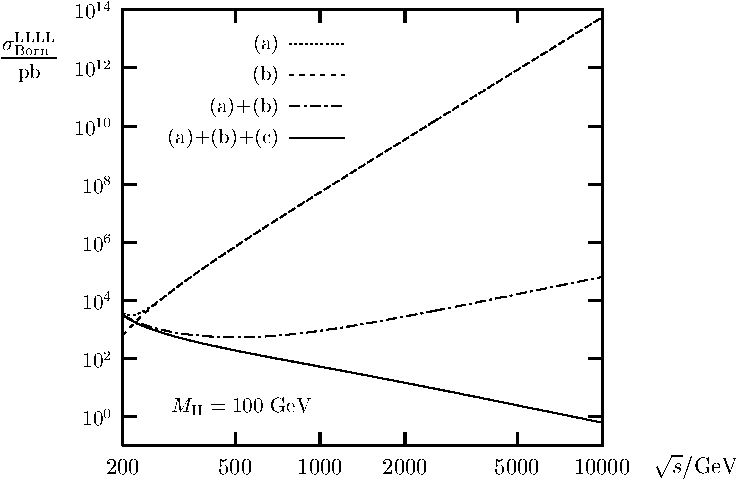
\includegraphics[width=0.7\textwidth]{figures/unitarity.pdf}
  \caption[The cross-sections for longitudinal polarized \gls{VBS} involving three
    and four-boson coupling with and without Higgs coupling included.]%
  {The cross-sections for longitudinal polarized \gls{VBS} involving three
    and four-boson coupling with and without Higgs coupling diagram included.
    (a) is for the diagrams with three-boson coupling,
    (b) is for diagrams with four-boson coupling, and (c) is for diagrams
    with Higgs to vector boson coupling.~\cite{Denner1997}}%
  \label{fig:vbs-at-high-energies}
\end{figure}

\subsection{
  Topology of VBS in Semileptonic ZV Final State
}

In proton-proton collisions, the actual interaction happens
with the constituent quarks. For \gls{VBS} to happen, the incoming
(colliding) quarks have to radiate vector boson, then the scattering
process between those vector boson can proceed via exchange of vector
boson, Higgs boson, or quartic coupling. The tree level Feynman
diagram of a VBS process in proton-proton
collision is shown in Figure~\ref{fig:feynman-vbs}.

The outgoing quarks are the signature of \gls{VBS} in hadron collider
experiments because they will have large pseudorapidity difference between
them, and will also have large invariant mass of outgoing quark pair.
Generally the jets
coming from these outgoing quarks are first tagged
as ``VBS Jets'' to filter out most of the \gls{QCD} background.

The type of leptonically decaying vector boson can be determined, i.e.
whether it was W or Z, but for the hadronically decaying vector
boson it is challenging and generally denoted by V.
This analysis looks for the \gls{VBS} signature with ZV in final state
with Z decaying to two \gls{OSSF} leptons, and V decaying to pair
of quarks.

\begin{figure}[!ht]
  \centering
  \begin{minipage}{0.5\textwidth}
    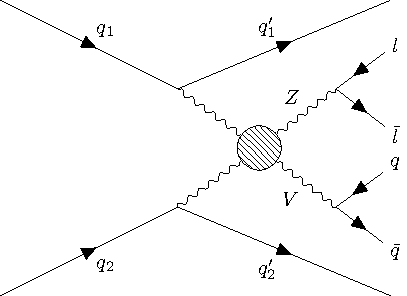
\includegraphics[width=\textwidth]{figures/feyn_vbs_0.pdf}
    \vspace{5pt}
  \end{minipage}
  \begin{minipage}{0.23\textwidth}
    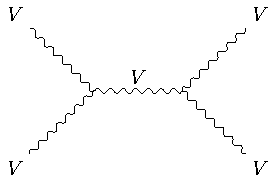
\includegraphics[width=\textwidth]{figures/feyn_vbs_2.pdf}
  \end{minipage}%
  \begin{minipage}{0.18\textwidth}
    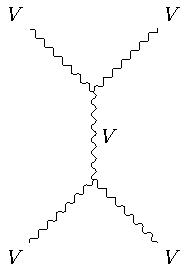
\includegraphics[width=\textwidth]{figures/feyn_vbs_4.pdf}
  \end{minipage}%
  \begin{minipage}{0.23\textwidth}
    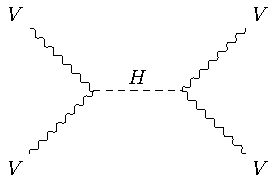
\includegraphics[width=\textwidth]{figures/feyn_vbs_3.pdf}
  \end{minipage}%
  \begin{minipage}{0.18\textwidth}
    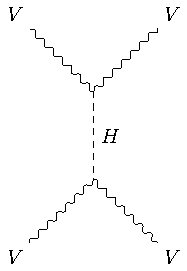
\includegraphics[width=\textwidth]{figures/feyn_vbs_5.pdf}
  \end{minipage}%
  \begin{minipage}{0.16\textwidth}
    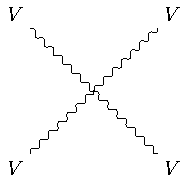
\includegraphics[width=\textwidth]{figures/feyn_vbs_1.pdf}
  \end{minipage}
  \caption[Tree level Feynman diagram of ZV VBS process at LHC]%
  {Tree level Feynman diagram of ZV VBS process at LHC\@. The top diagram
    shows the production of two vector boson being radiated from incoming
    quarks, in final state after scattering (blob), Z decays
    to pair of leptons, V (W/Z) decays to pair of quarks,
    and plus two outgoing quarks.
    The bottom row of diagram shows the tree
    level processes that can happen in scattering represented by blob in
    top diagram, starting from s and t-channel exchange of
    vector boson, Higgs boson, and the last one is quartic
    coupling of vector bosons.
  }%
  \label{fig:feynman-vbs}
\end{figure}
\chapter{
  The LHC and CMS Experiment
 }\label{experiment}

\section{
  LHC
 }\label{experiment:lhc}

About \gls{LHC}

\section{
  CMS
 }\label{experiment:cms}

About \gls{CMS} experiment

\subsection{
  Calorimeter and HGCAL Upgrade
}

About Calorimeter and \gls{HGCAL} Upgrade

\subsection{
  Tracker System
}

About \gls{CMS} Tracker System
\chapter{
  Chapter 3
 }\label{chap3}

\chapter{
  Chapter 4
 }\label{chap4}

\chapter{
  Chapter 5
 }\label{chap5}


% References
\printbibliography[heading=bibintoc, title={References}]

% Appendices
\appendix
\chapter{
  Analysis Code
 }


Analysis code used for the analysis is hosted on
Github (\url{https://github.com}) platform.

\begin{itemize}
  \item Custom NanoAOD production from MiniAOD
        to include missing \gls{PDF} weights.

        \url{https://github.com/singh-ramanpreet/VBS-customNanoAODProduction/}

  \item ``NanoSkim'': Intermediate skimming step for the analysis
        phase space with minimal selection to save time,
        when run it again during analysis development.

        \url{https://github.com/singh-ramanpreet/VVjjSemileptonic-NanoSkim}

  \item ``Selection'': This repo contains the code for main event
        selection of this analysis, it also calculates and embed scale factors
        for various objects.

        \url{https://github.com/singh-ramanpreet/VVjjSemileptonic-Selection}

  \item ``Analysis'': This repo contains code \gls{MVA} training,
        \gls{MVA} inference and embedding, making Data/MC histograms,
        making datacards for the statistical analysis with \texttt{CombineLimit}.

        \url{https://github.com/singh-ramanpreet/VVjjSemileptonic-Analysis}

\end{itemize}

\chapter{
  Additional Kinematic Distributions
 }

Add backup plots.

\end{document}